\chapter{準備}

本章では,次章以降で必要となる事項について説明する.

\section{数理計画問題}

数理計画問題は以下のように表すことができる\cite{数理計画入門}:\\
         目的関数 : $f(x)$ → 最小(あるいは最大)\\
         制約条件 : $ x \in S$\\
ここで,$x$は$n$次元実ベクトル,目的関数$f$は$R^n$($n$次元実ベクトル空間)上で定義された実数値関数である.
また制約条件を満たす$x$を実行可能解,その集合である$S \subseteq R^n$を実行可能領域,実行可能解のなかで目的関数$f(x)$が最小(あるいは最大)となるものを最適解という.
このような問題を総称して数理計画問題(最適化問題)という.

\section{分枝限定法}

分枝限定法とは組合せ最適化問題の解を見つける方法の1つである\cite{数理計画入門, ハンドブック}.
組合せ最適化問題は有限個の要素からなる実行可能領域のなかで目的関数が最小となる解を見つける問題である.
実行可能解は有限個であるから,それらすべてを列挙することにより,最適解を求めることができる.
しかしながら,変数の数が多い場合,組合せの数が膨大になるため,すべての実行可能解を比較する方法では最適解を求めるのは難しい.

これに対し,分岐限定法は組み合わせ最適化問題の最適解を効率的に見つけるための方法のひとつである.
分枝限定法において,実行可能解を列挙するために場合分けを行っていく過程で,最適解が得られる見込みのない不必要な場合分けをできるだけ省略して探索する範囲を絞り込み,計算時間の短縮を図る.
分枝限定法の探索の方法を以下に記述する.
ここで,下界値とは最適値以下であることがわかっている値であり,上界値とは最適値以上であることが分かっている値である.

\begin{itembox}[l]{分枝限定法}
\begin{description}
\item[ステップ1] 適切な方法で初期実行可能解を求め,それを暫定解$x$とする.
暫定解$x$の目的関数値を$z$とする.
問題の集合${\cal N}={P_0}$とする($P_0$は原問題である).
\item[ステップ2] ${\cal N}=0$ならば,暫定解$x$を最適解として出力し終了.\\
そうでなければ,${\cal N}$から適当な子問題を選びそれを$P'$とし,${\cal N}$から$P'$を取り除く.
\item[ステップ3] $P'$の緩和問題を解き,得られた解を$\bar{x'}$,上界値を$\bar{z'}$とする.
緩和問題が許容解をもたないならばステップ2へ.
\item[ステップ4] $\bar{x'}$が元問題$P_0$の実行可能解かつ$\bar{z'}>z$の場合.\\
(原問題$P_0$の,より良い許容解が得られたので)$x:=\bar{x'}$,  $z:=\bar{z'}$と更新する.
ステップ2へ.
\item[ステップ5] $\bar{z'} \leq z$の場合.\\
(子問題$P'$の最適解は$x$より目的関数値が大きくないので)ステップ2へ.
\item[ステップ6] ($\bar{x'}$が元問題$P_0$の実行可能解でない,かつ$\bar{z'} > z$の場合)\\
$P'$の実行可能領域を分割した子問題を生成し,それらを${\cal N}$に加え,ステップ2へ.
\end{description}
\end{itembox}


\section{割当問題}

まず,割当問題の説明を行う際に必要となるマッチング問題について説明する.
マッチング問題とは,複数の仕事と複数の機械を1対1に対応させたり,何人かの人を2人ずつのグループに分けたりするように,対象物のペアを作る問題である.
この問題は,無向グラフ上でモデル化できる.
モデル化する際に,対象を頂点とし,ペアリング可能な頂点同士を無向枝で結ぶ.
ここで,ペアを作る枝の集合をマッチングという.
このようにして,要素数最大のマッチングか,各枝に与えられた費用の和が最小となる条件を満たすマッチングを求める問題をマッチング問題という.
そして,マッチング問題の中でも,2部グラフの最小費用マッチング問題を割当問題\cite{ハンドブック}と呼ぶ.
例えば,能力が異なる各社員にどの作業を割り当てると最もコストが少なくなる(もしくは最も利益を上げることができる)のかを求める問題を考える.
その例を図\ref{fig:wariate}に示す.
この図の点線はマッチング可能なペアを表しており,実線はマッチングを表している.
すなわち,社員a1が仕事b2, b3に割り当てられ,社員a2が仕事b4に割り当てられ,社員a3が仕事b1に割り当てられている\cite{ハンドブック}.
\begin{figure}[h]
\centering
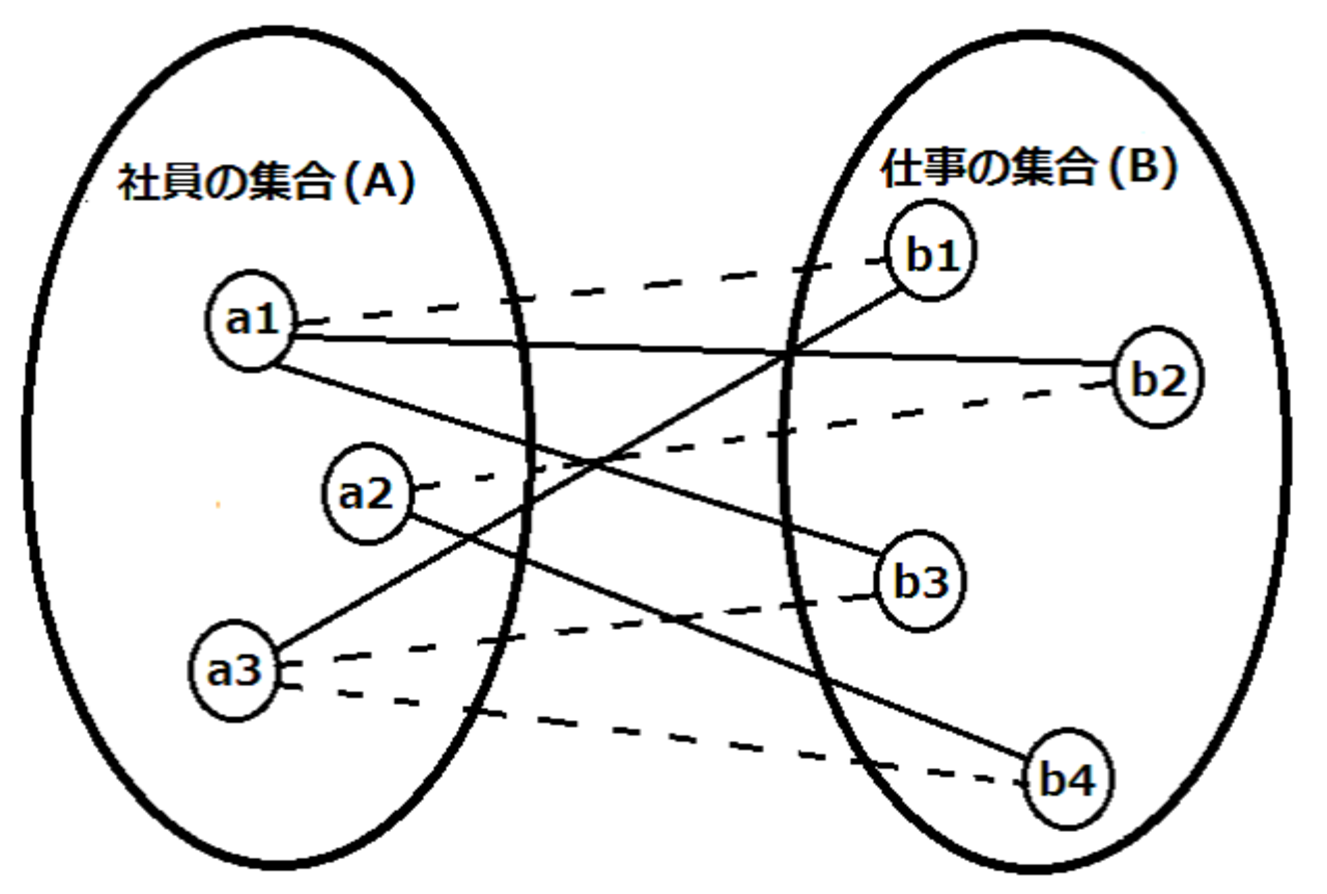
\includegraphics[width=10cm, clip]{wariate.eps}
\caption{割当問題の例}
\label{fig:wariate}
\end{figure}



\section{重み付き制約充足問題(WCSP)}

制約充足問題 (Constraint Satisfaction Problem, CSP)とは,変数の集合,変数領域の集合,制約の集合によって構成され,すべての制約を満たすように各変数に変数領域から値を割り当てる問題である.
このとき,すべての制約が満たされた解を実行可能解と呼ぶ.
一方,WCSP (Weighted CSP)\cite{CSP}では重要な制約条件をなるべく満足するためには値をどのように割り当てるとよいかを決定する問題であり,すべての制約を満たす必要はなく,制約条件の重要度を重みとして設定することができる.
そのため,制約条件は大きく2種類に分類することができる.
1つが絶対制約で,これは必ず成立させなければならない制約条件である.
よって,この制約が1つでも成り立っていない解は実行可能解とは言えない.
もう1つが考慮制約で,これは成立させることが好ましい制約条件である.
この制約が成り立っていない解も実行可能解と言える.
このとき,各考慮制約毎に違反ポイントを設定し,その総和を目的関数として,それを最小化する.


\section{最適化ソルバー}

最適化ソルバーは,数理計画問題の最適解を得るためのプログラムである.
これを利用するためにはまず,数理計画問題の定式化を行い,次に定式化した問題をモデリング言語で記述する.
最適化ソルバーによって利用できるモデリング言語は異なる.
そして,記述した問題を最適化ソルバーで読み込み,解を得る.
ここで,本研究で用いる最適化ソルバーGLPK\cite{GLPK}とIBM ILOG CPLEX Optimizer\cite{CPLEX}について説明する.

まずGLPKとは,GNU Linear Programming Kit の略で,GNUが無料配布しているソルバーである.
GLPKは,モデリング言語として,最適化の分野で広く用いられているモデリング言語AMPL (A Mathematical Programming Language)\cite{AMPL}のサブセット言語であるGMPLを採用している.
このソルバーは最適化計算を行うだけではなく,GMPL形式で書かれたモデルとデータを用いて,LP形式のファイルを作成することができる.

また,IBM ILOG CPLEX Optimizer\cite{CPLEX}とは,計算速度に定評のある最適化ソルバーの1つである.
モデリング言語はOPLを採用している.
そして,大規模な線形計画(LP),2次計画(QP),整数計画(IP),混合整数計画(MIP)を解くことができる.

本研究では,GLPKによって,GMPL形式で書かれたモデルとデータを,LP形式のファイルへ変換し,IBM ILOG CPLEX Optimizerを用いて計算を行っている.
